\documentclass{standalone}
\usepackage{tikz}
\usepackage{tikz-qtree}

\begin{document}

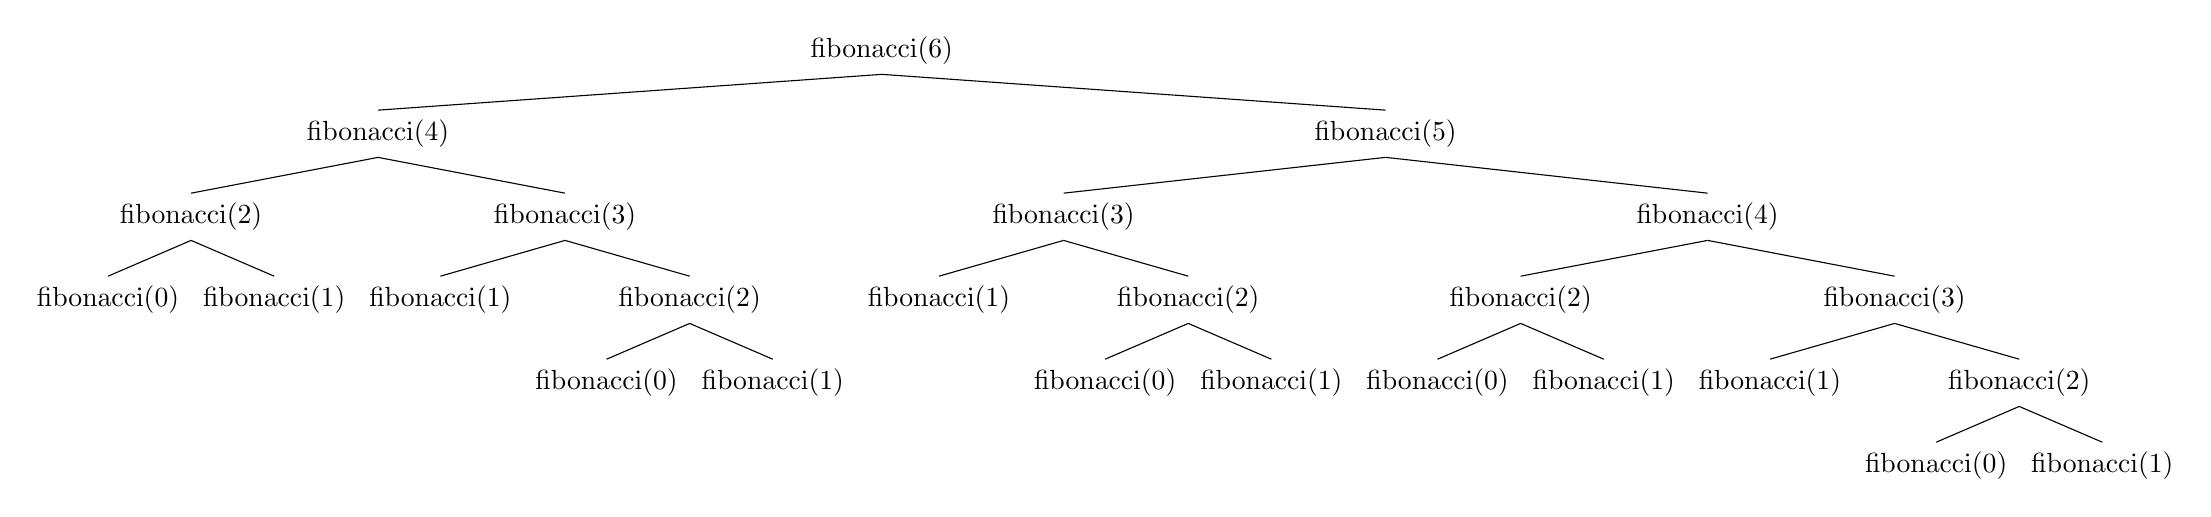
\begin{tikzpicture}
\Tree
[.fibonacci(6)
    [.fibonacci(4)
        [.fibonacci(2)
            [.fibonacci(0) ]
            [.fibonacci(1) ]
        ]
        [.fibonacci(3)
            [.fibonacci(1) ]
            [.fibonacci(2)
                [.fibonacci(0) ]
                [.fibonacci(1) ]
            ]
        ]
    ]
    [.fibonacci(5)
        [.fibonacci(3)
            [.fibonacci(1) ]
            [.fibonacci(2)
                [.fibonacci(0) ]
                [.fibonacci(1) ]
            ]
        ]
        [.fibonacci(4)
            [.fibonacci(2)
                [.fibonacci(0) ]
                [.fibonacci(1) ]
            ]
            [.fibonacci(3)
                [.fibonacci(1) ]
                [.fibonacci(2)
                    [.fibonacci(0) ]
                    [.fibonacci(1) ]
                ]
            ]
        ]
    ]
]
\end{tikzpicture}

\end{document}